\documentclass{article}
\usepackage[pdfcreator={LaTeX}]{hyperref}
\usepackage{graphicx}
\usepackage[utf8]{inputenc} 
\usepackage[ngerman]{babel}


\usepackage{tikz}
\usetikzlibrary{arrows,shadows}
\usepackage{pgf-umlsd}


\begin{document}
\begin{titlepage}

\begin{center}
\textbf{\textsc{\LARGE Implementierungsbericht}}

{\large \today}

\vspace{2cm}
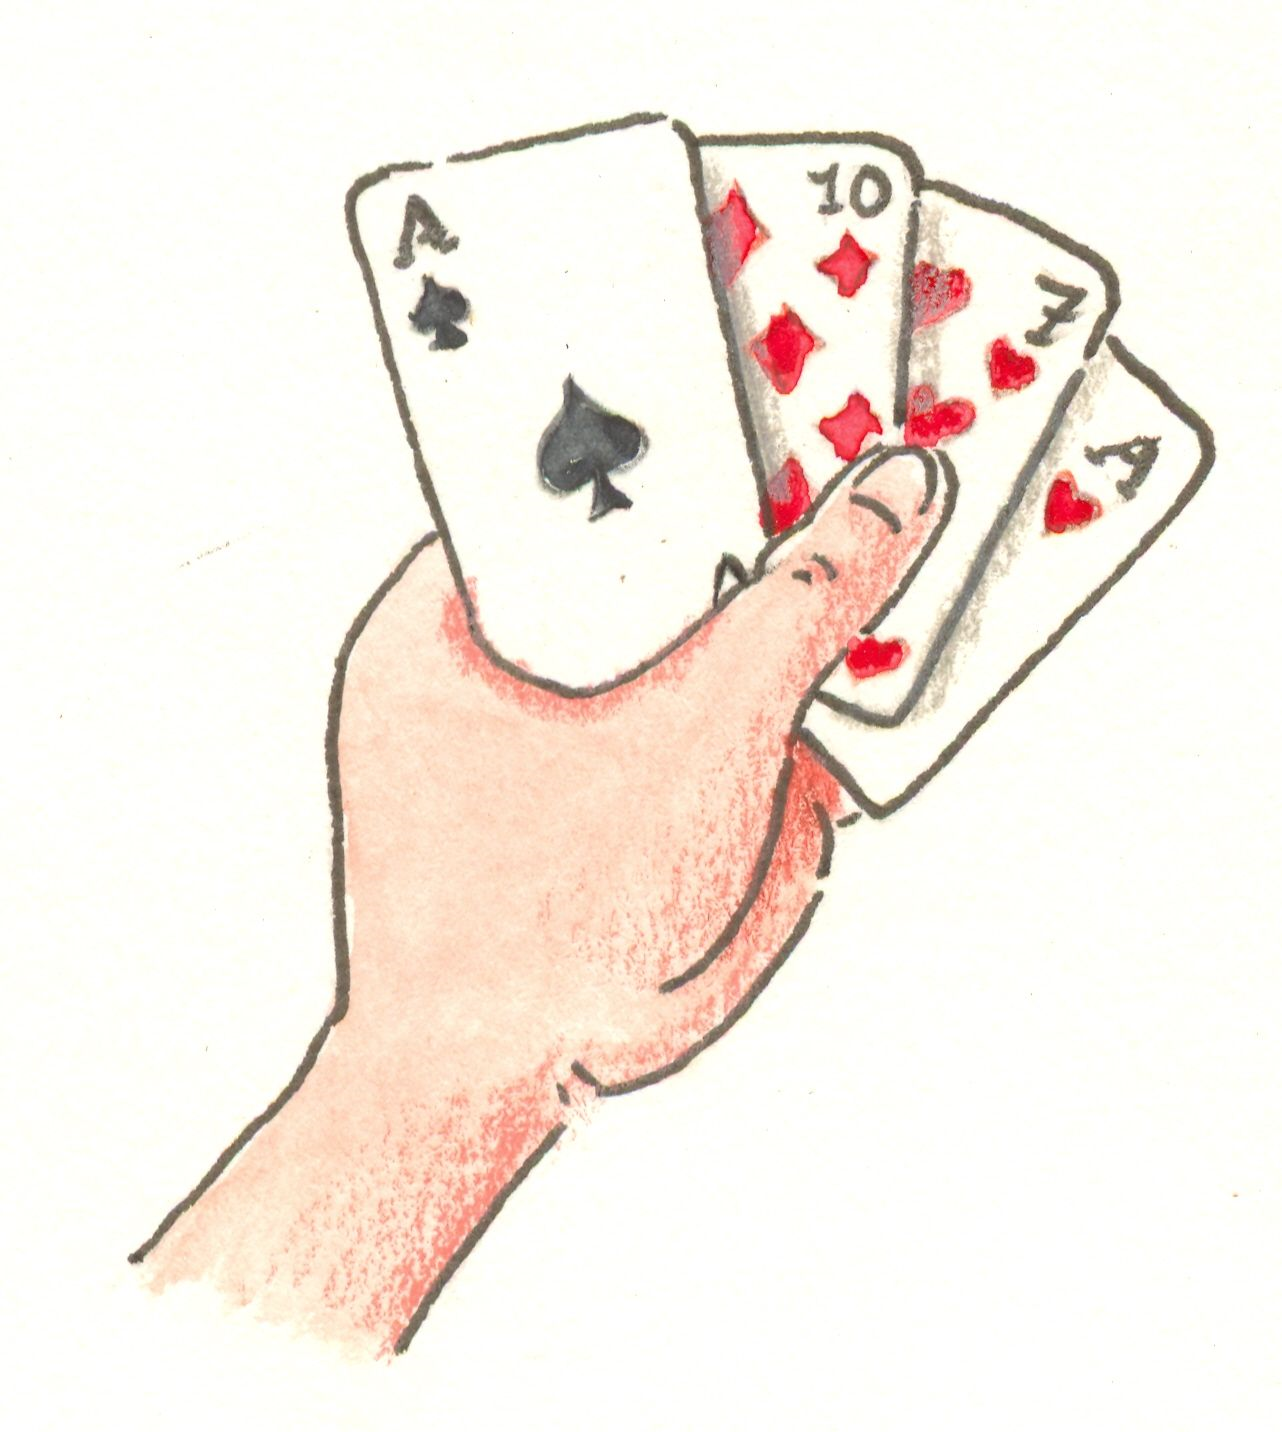
\includegraphics{kartenspiel}
\ \\
\ \\

\textbf{\textsc{\LARGE NET-WizHearts}}
\vspace{2cm}

\begin{tabular}{|c|c|c|}\hline
   Phase & Verantwortlicher & E-Mail \\ \hline\hline
   Pflichtenheft & Alina Meixl &  alina@meixl.de \\ \hline
   Entwurf & Viktoria Witka & witkaviktoria@freenet.de \\ \hline
   Spezifikation & Daniel Riedl & dariedl14@yahoo.de \\ \hline
   Implementation & Andreas Altenbuchner& a.andi007@gmail.com\\ \hline
   Verifikation & Patrick Kubin & kubin@fim.uni-passau.de\\ \hline
   Präsentation & w& w\\ \hline
 \end{tabular}

\end{center}

\end{titlepage}

\tableofcontents
\newpage

\section{Einleitung}
Hier kommt die Implementierung

\newpage

\section{Änderungen gegenüber der Spezifikation}

\subsection{Client}

\begin{itemize}
\item 
\end{itemize}

\subsection{View}

\begin{itemize}
\item Login: Methoden getUsername(), getServerAdress() hinzugefügt
\item Lobby: Methoden getChosenGameName(), getChatMessage() hinzugefügt
\end{itemize}

\subsection{Ruleset}

\begin{itemize}
\item 
\end{itemize}

\subsection{Server}

\begin{itemize}
\item 
\end{itemize}

\subsection{ComObjects}

\begin{itemize}
\item 
\end{itemize}

\newpage

\section{Vergleich: Implementierungsplan und Realität}

\subsection{Milestone 1}

\begin{itemize}
\item View(Login+Lobby): ang. Dauer: 8 Stunden, tats. Dauer: 4 Stunden \\
Begründung: Es waren noch Code-Teile aus der Pflichtenheft-Phase vorhanden.
\end{itemize}

\subsection{Milestone 2}

\subsection{Milestone 3}

\subsection{Finale Phase}




\end{document}
